\section{Parsing the \oeis Formula Format}\label{sec:form-parser}
We built a partial parser for \oeis formulas by identifying
and analyzing well-behaved formulas to produce a workable grammar.
We leverage the fact that, although there is no standardized format for \oeis formulas, many of them use a
sufficiently
regular syntax.

\oeis is known for the human-readable mathematical terms, so a variety of syntactic rules are encountered when forming
these mathematical terms. We use the following classification for notations, inspired by \cite{ranta} and
further motivated by our analysis of the \oeis formulas:
\begin{compactenum}
\item \textbf{infix operators} are used to combine two terms to one complex term, e.g the \lstinline!+! symbol in
\lstinline!m+n!.
\item \textbf{suffix operators} are added after a term to form another term, e.g. the \lstinline|!| symbol in
\lstinline|n!|.
\item \textbf{prefix operators} (with or without bracketed application) are added in front of a term to form another
term,
e.g. \lstinline|sin| in \lstinline|sin(x)| or \lstinline|sin x|, respectively.
\item \textbf{infix relation symbols} are used to construct a formula out of two terms, e.g. the \lstinline|<| symbol
in \lstinline|x<2|.
\item \textbf{binding operators} that bind a context to a body to construct a term, e.g. the
\lstinline[mathescape]|$\forall$| symbol in
\lstinline[mathescape]|$\forall$x. x^2 > 0|
\end{compactenum}

The classification presented above guides our grammar and, in principle, covers virtually all important notations used
in \oeis formulas. However, in practice, we encountered several important challenges which we discuss individually
below.

\paragraph{Open Set of Primitives} Since the formulas are not standardized, not only is
the syntax flexible, but so is the set of primitive operators that are used. For instance,
the formulas in Listing \ref{lst:internal} (on lines $5$-$6$) use square root, power, as
well as the sum (\lstinline[mathescape]|$\Sigma$|) and product
(\lstinline[mathescape]|$\Pi$|) binders. The challenges arise because of the many
different notations used for such primitives. For instance, in line $6$ of Listing
\ref{lst:internal} the range for sum and product is given in two different ways. Similar
problems appear with limits and integrals as well as numerous atypical infix and suffix
operators.  In order to parse these correctly, we investigate the documents and the
grammar failures manually and incrementally extend the grammar.

\paragraph{Ambiguity}
As it is often the case with informal, presentation-oriented formulas, there can be
ambiguity in the parsing process when there exist several reasonable
interpretations. Since the \oeis syntax is not fixed, this is quite common, so we do
additional disambiguation during parsing to resolve most of the ambiguities. Here we
discuss a few of the many ambiguities that arise.

The multiplication sign is usually implicit so, instead of \lstinline!a*(x+y)!, we
encounter \lstinline!a(x+y)! which could represent either a function application or a
multiplication depending on whether \lstinline!a! is a function or an individual (constant
or variable).  There is no general way to solve this, so we rely on several
heuristics. First, we check if the symbol in question is used somewhere else in the same
formula with an unambiguous meaning.  Specifically, we default to function application
unless the same symbol is used as an individual somewhere else in the formula. This
already disambiguates most such cases in \oeis but we use several additional
heuristics. For instance, having \lstinline[mathescape]!name($arg$)! will result in
marking \lstinline!name! as function since it is unlikely to be a multiplication between
two individuals. Similarly, having \lstinline[mathescape]!name($arg_1$,...,$arg_n$)!
results in marking \lstinline!name! as a function.

The natural way of using the power operator also leads to ambiguities. For example,
\lstinline!T^2(y)! is used for $(T(y))^2$, however \lstinline!T^y(x^2+2)! is ambiguous.
We solve this using similar heuristics as for the implicit multiplication.

For unbracketed function application as in \lstinline!sin x!, we rely on the heuristic that this form of function
application is used only in well known functions. Therefore, we code these notations for well known
functions in the grammar itself. This form of function application can also mean multiplication, for instance
\lstinline!Pi x!.
One can already see that parsing and disambiguating the mathematical expressions in this context has a lot of aspects.
Additional cases of ambiguities are handled in similar ways and we omit the details for brevity.

\paragraph{Delineating formulas}
\oeis formula lines freely mix text and formulas so it is required to correctly distinguish between text and formula
parts within the lines in order to accurately parse each line. For instance, line $6$ in Listing
\ref{lst:internal} starts with the text \lstinline!G.f.:! (meaning ``Generating function:'') and continues with the
formula. The line then has the author and date, separated from the formula by a dash (\lstinline!-!) which
could also be interpreted as a minus and, therefore, a continuation of the formula.
In the extraction of the formulas we use the help of a dictionary. The text in the \oeis documents has words
that are not found in the dictionaries since it contains many technical terms so we first run a
pre-parsing procedure which enriches the dictionary. The final grammar tries to parse words until it fails and then
tries to parse formulas; this process repeats.

\subsection{Importing into \omdmmt}
For each \oeis document we create a corresponding \omdmmt document that contains a single theory. Then, \oeis lines
roughly correspond to \omdmmt declarations inside that theory. We use the \oeis sequence ID as the name of the \omdoc
theory. Then, the identification line produces an \omdoc symbol declaration representing the sequence (as a function
from integers to values). The start values and example lines are both represented as \omdmmt examples. Specifically,
the starting values are considered as examples of sequence elements. Formula lines are represented as \omdoc
assertions
(about the sequence symbol). Finally, name, reference and author lines are represented as metadata using the Dublin
Core standard.

[Fibonacci Numbers]\label{ex:omdoc}
 The corresponding \omdmmt document for the Fibonacci numbers article from Example \ref{ex:internal} is shown
 in Listing \ref{lst:omdoc}. We omit most formulas and some XML boilerplate for conciseness and simplicity.

 \begin{lstlisting}[mathescape,label=lst:omdoc]
  <omdoc xmlns:dc="http://purl.org/dc/elements/1.1/">
    <theory id="A000045">
    <metadata>
      <dc:creator>N. J. A. Sloane</dc:creator>
      <dc:title>Fibonacci numbers</dc:title>
    </metadata>
    <symbol name="seq"/>
    <assertion>
      <!-- OpenMath for $\forall n. seq(n) = \frac{(1 + \sqrt{5})^n - (1 - \sqrt{5})^n}{2^n \sqrt{5}}$ -->
      <OMBIND>
        <OMS cd="arith" name="forall"/>
        <OMBVAR> <OMV name="n"/> </OMBVAR>
        <OMA>
          <OMS cd="arith" name="equal"/>
          <OMA><OMS name="seq"/><OMV name="n"></OMA>
          $\vdots$
        </OMA>
      </OMBIND>
    </assertion>
    $\vdots$
    </theory>
  </omdoc>
 \end{lstlisting}


\subsection{Implementation and Evaluation}
The importer is implemented in Scala as an extension for the \mmt system and consists of about 2000 lines of code.
It is available at \url{https://svn.kwarc.info/repos/MMT/src/mmt-oeis/}. The implementation is mostly straightforward,
other than the formula parser which we discuss separately below.

There are $257654$ documents in \oeis totaling over $280$MB of data. The \omdmmt import expands it to around
$9$GB,
partly due to the verbosity of XML and partly due to producing the semantic representation of formulas.
The total running time is around $1$h$40$m  using an Intel Core i5, $16$GB of RAM and a SATA hard drive.

\paragraph{Formula parsing} The formula parser is implemented using the Packrat Parser \cite{packrat} for which Scala
provides a standard implementation. Packrat parsers allow us to write left recursive grammars while guaranteeing a
linear time worst case which is important for scaling to the \oeis.

 There are $223866$ formula lines in \oeis and the formula parser succeeds on $201384$ (or
$90\%$) of them. Out of that, $196515$ (or $97.6\%$) contain mathematical expressions.
Based on a manual inspection of selected formulas we determined that most parser fails occur because of
logical connectives since those are not yet supported. Other failures include
wrong formula delineation because of unusual mix of formulas and text.

The statistics above refer just to the successful parses, but we cannot automatically evaluate if the result
returned by the parser is actually the expected one. For this, we did a manual evaluation of the parsing result for
$40$ randomly selected \oeis documents and evaluated $85$\% of successfully
parsed formulas as semantically correct. The main contributor of incorrect formula parses was badly delineated
formulas, which causes text to be wrongly parsed as part of a formula.

\section{Search} \label{sec:Search}
%\subsection{Realizing Text and Formula search for \oeis}

{\mws} (\mwss)\cite{KohPro:man13} is an open-source, open-format, content-oriented search engine for mathematical
expressions. We refer to \cite{KohPro:man13} for details.

To realize the search instance in \mwss we need to provide two things:
\begin{compactenum}
 \item A \emph{harvest} of \mathml-enriched \html files that the search system can resolve queries against.
 The content-\mathml from the files will be used to resolve the formula part of the query while the rest of the \html
will be used for the text part. The harvest additionally requires a configuration file
that defines the location in the \html files of \mwss-relevant metadata such as the title, author or URL of the
original
article. This, together with the \html itself is used when presenting the query results.
 \item A \emph{formula converter} that converts a text-based formula format into \mathml. This will be used so that
 we can input formulas for searching in a text format (in our case \oeis-inspired ASCII math syntax) rather than
 writing
 \mathml directly.
\end{compactenum}

\begin{figure}
\centering
 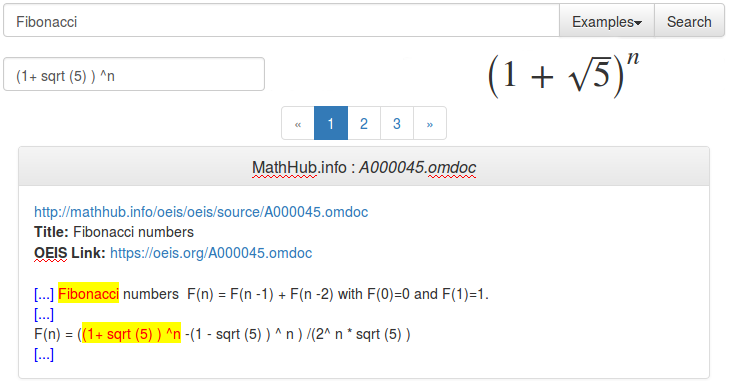
\includegraphics[scale=0.45]{search.png}
 \caption{Text and Formula Search for \oeis}\label{fig:search}
\end{figure}

To produce the harvest of the \oeis library for \mwss we export the \html from the content imported
into \mmt. We reuse the \mmt presentation framework and only enhance it with \oeis-specific technicalities such as
sequence name or \oeis link. For the formula converter we use the same parser used for \oeis formulas and described
above, except extended with one
grammar rule for \mwss \emph{query variables}. We then forward the resulting formula in \mmt to produce the
presentation
(\mathml) and return it to the \mwss frontend.  The web-server infrastructure, needed to communicate with \mwss, is
provided
by \mmt and we just extend it. Figure \ref{fig:search} shows (a part of) the current interface answering a query about
Fibonacci numbers. The search system is available at \url{http://ash.eecs.jacobs-university.de:9999/}.



%%% Local Variables:
%%% mode: latex
%%% TeX-master: "report"
%%% End:
